
%(BEGIN_QUESTION)
% Copyright 2011, Tony R. Kuphaldt, released under the Creative Commons Attribution License (v 1.0)
% This means you may do almost anything with this work of mine, so long as you give me proper credit

Once upon a time, an instrument technician (and BTC graduate!) stumbled upon this temperature measurement circuit at a biopharmaceutical manufacturing facility, used to measure the temperature of storage freezers:

$$\includegraphics[width=15.5cm]{i03740x01.eps}$$

Identify the type of calibration error introduced by this improper wiring (e.g. zero shift, span shift, linearity, hysteresis), and also explain how the wiring error may be corrected for improved measurement accuracy.

\underbar{file i03740}
%(END_QUESTION)





%(BEGIN_ANSWER)


%(END_ANSWER)





%(BEGIN_NOTES)

You will never realize the benefits of a four-wire RTD circuit until you actually use it as a four-wire RTD, not a glorified two-wire RTD as was the case with the original circuit!

$$\includegraphics[width=15.5cm]{i03740x02.eps}$$

With the original circuit, wire resistance would not have been compensated for, leading to a {\it zero shift} calibration error.  The transmitter would have ``thought'' the RTD was warmer than it actually was by the amount equivalent to the wires' added resistance.

\vskip 10pt

Interestingly, after this wiring error was identified, it was determined that it could not be corrected because it was part of a designed process at the biopharmaceutical facility and therefore all design details (including the incorrect wiring) were ``locked'' and could not be altered without an entire re-evaluation of the process.  This is an example of a strict MOC (Management Of Change) policy where changes possibly influential to the operation of a process must go through an extensive review before being implemented.

%INDEX% Measurement, temperature: RTD

%(END_NOTES)

